\section{Task 1: TLS Client}
\subsection{Task 1.a: TLS handshake}
%
I used the command below to communicate with {\fontfamily{qcr}\selectfont tuni.fi}
server.

\begin{lstlisting}[language=bash]
    python3 handshake.py tuni.fi
\end{lstlisting}

\begin{lstlisting}[caption=A TLS hanshake connecting to \url{www.tuni.fi}.,
    label={lst:handshake_log}]
Cipher used: ('ECDHE-RSA-AES128-GCM-SHA256', 'TLSv1.2', 128)
=== Server hostname: tuni.fi
=== Server certificate:
{'OCSP': ('http://GEANT.ocsp.sectigo.com',),
 'caIssuers': ('http://GEANT.crt.sectigo.com/GEANTOVRSACA4.crt',),
 'crlDistributionPoints': ('http://GEANT.crl.sectigo.com/GEANTOVRSACA4.crl',),
 'issuer': ((('countryName', 'NL'),),
            (('organizationName', 'GEANT Vereniging'),),
            (('commonName', 'GEANT OV RSA CA 4'),)),
 'notAfter': 'Jun 21 23:59:59 2023 GMT',
 'notBefore': 'Jun 21 00:00:00 2022 GMT',
 'serialNumber': '169B2623CE1AFC3A7FDDDFD89EB7437E',
 'subject': ((('countryName', 'FI'),),
             (('stateOrProvinceName', 'Pirkanmaa'),),
             (('organizationName', 'Tampere University Foundation sr'),),
             (('commonName', 'www.tuni.fi'),)),
 'subjectAltName': (('DNS', 'www.tuni.fi'), ('DNS', 'tuni.fi')),
 'version': 3}
[{'issuer': ((('countryName', 'US'),),
             (('stateOrProvinceName', 'New Jersey'),),
             (('localityName', 'Jersey City'),),
             (('organizationName', 'The USERTRUST Network'),),
             (('commonName', 'USERTrust RSA Certification Authority'),)),
  'notAfter': 'Jan 18 23:59:59 2038 GMT',
  'notBefore': 'Feb  1 00:00:00 2010 GMT',
  'serialNumber': '01FD6D30FCA3CA51A81BBC640E35032D',
  'subject': ((('countryName', 'US'),),
  (('stateOrProvinceName', 'New Jersey'),),
  (('localityName', 'Jersey City'),),
  (('organizationName', 'The USERTRUST Network'),),
  (('commonName', 'USERTrust RSA Certification Authority'),)),
    'notAfter': 'Jan 18 23:59:59 2038 GMT',
    'notBefore': 'Feb  1 00:00:00 2010 GMT',
    'serialNumber': '01FD6D30FCA3CA51A81BBC640E35032D',
    'subject': ((('countryName', 'US'),),
    (('stateOrProvinceName', 'New Jersey'),),
    (('localityName', 'Jersey City'),),
    (('organizationName', 'The USERTRUST Network'),),
    (('commonName', 'USERTrust RSA Certification Authority'),)),
    'version': 3}]
\end{lstlisting}

The agreed ciphersuite and the server certificate are shown in
\autoref{lst:handshake_log}. The agreed ciphersuite is ``ECDHE-RSA-AES128-GCM-SHA256'',
which means that:

\begin{itemize}
    \item Key Exchange: Elliptic Curve Diffie-Hellman Ephemeral (ECDHE).
    \item Authentication (Public-Key Digital Signature): Rivest Shamir Adleman algorithm (RSA).
    \item Encryption: Advanced Encryption Standard with 128bit key in Galois Counter mode
    (AES128-GCM).
    \item Hash: Secure Hash Algorithm 256 (SHA256)
\end{itemize}


{\fontfamily{qcr}\selectfont /etc/ssl/certs}
is the directory storing CA certificates used to validate other peers' certificates.

%%% List of figures showing TCP and TLS packets
\begin{figure}
    \centering
    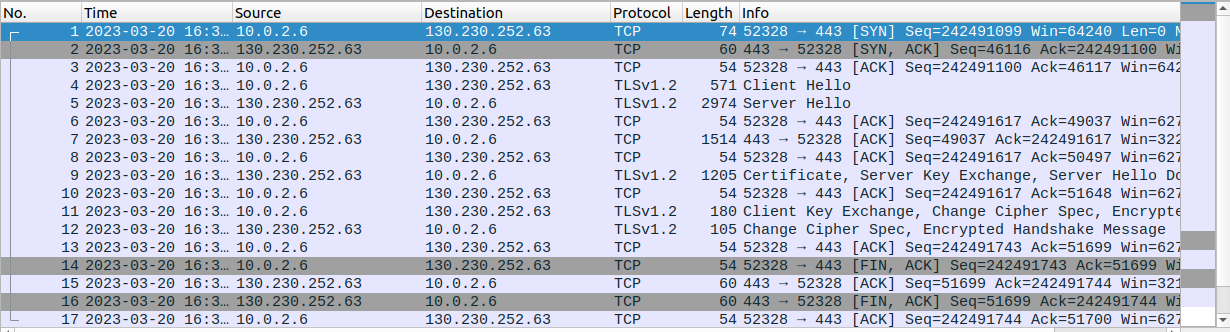
\includegraphics[height=\textheight,width=\textwidth,keepaspectratio]
    {figures/wireshark_packets.png}
    \caption{All TCP and TLS packets were transmitted while
    {\fontfamily{qcr}\selectfont handshake.py} was running.}
    \label{fig:all_packets}
\end{figure}


%%% End of figures listing

Some clarification:
\begin{itemize}
    \item Host machine IP address: 10.0.2.6
    \item {\fontfamily{qcr}\selectfont tuni.fi} server IP address: 130.230.252.63
\end{itemize}

As TLS is built on top of the Transmission Control Protocol (TCP), there had been a TCP 3-way
handshake before a TLS was initialized (see \autoref{fig:all_packets}).Firstly, the client
sent a segment with SYN to the web server and with a \emph{Seq} number (242491099)
for initializing a communication. Then, the server responded with a SYN-ACK with a pair of
\emph{Seq} and \emph{Ack} number. In the response, \emph{Ack} is the one-incremented number
of the previous \emph{Seq} number (242491100) in the initializing request, and the new \emph{Seq} number
here (46116) was generated by the server. Finally, after receiving the SYN-ACK signal, the client
sent back the ACK with the \emph{Seq} number which equals to the previous \emph{Ack} number (242491100)
and the \emph{Ack} number which is a one-incremented of the previous \emph{Seq} number (46117).
So the TCP 3-way handshake protocol ended here.

\begin{figure}
    \centering
    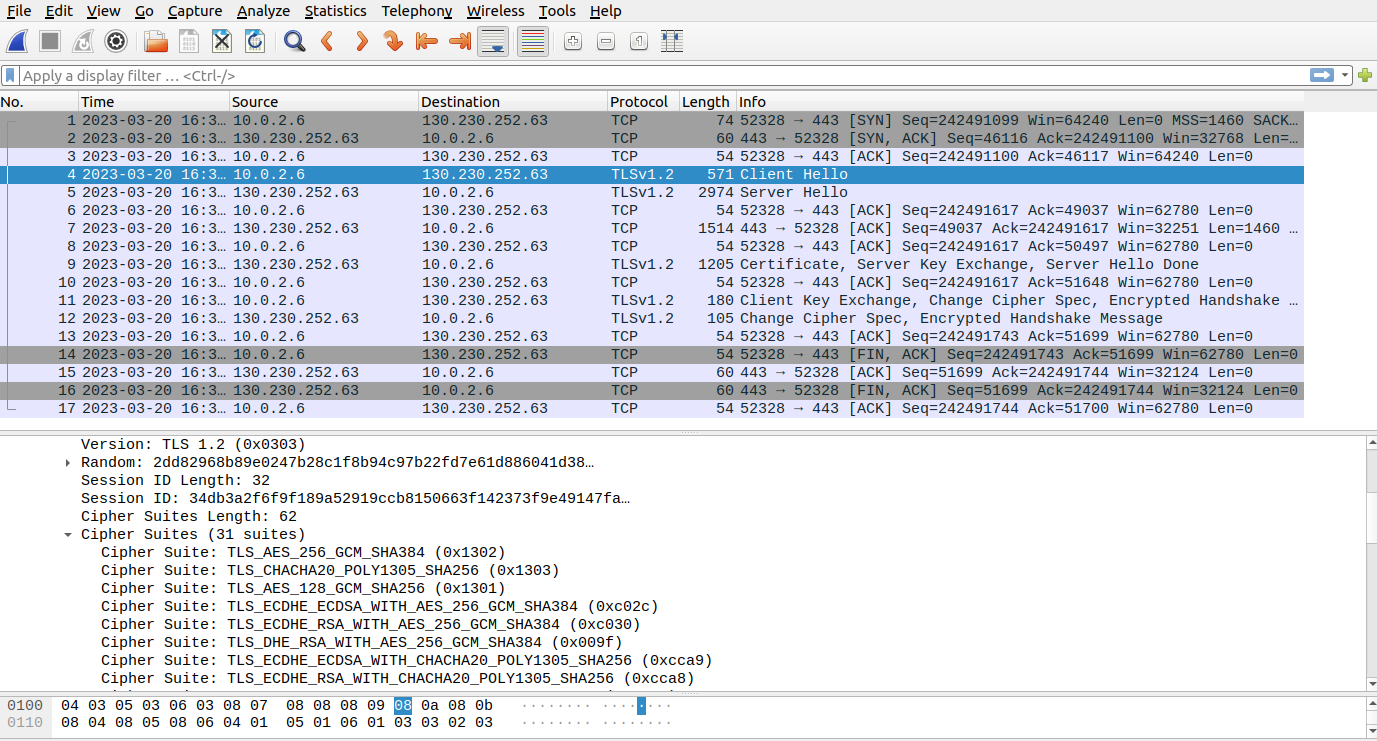
\includegraphics[height=\textheight,width=\textwidth,keepaspectratio]
    {figures/client_hello.png}
    \caption{`Client Hello' message of a TLS handshake.}
    \label{fig:client_hello_handshake}
\end{figure}

\begin{figure}
    \centering
    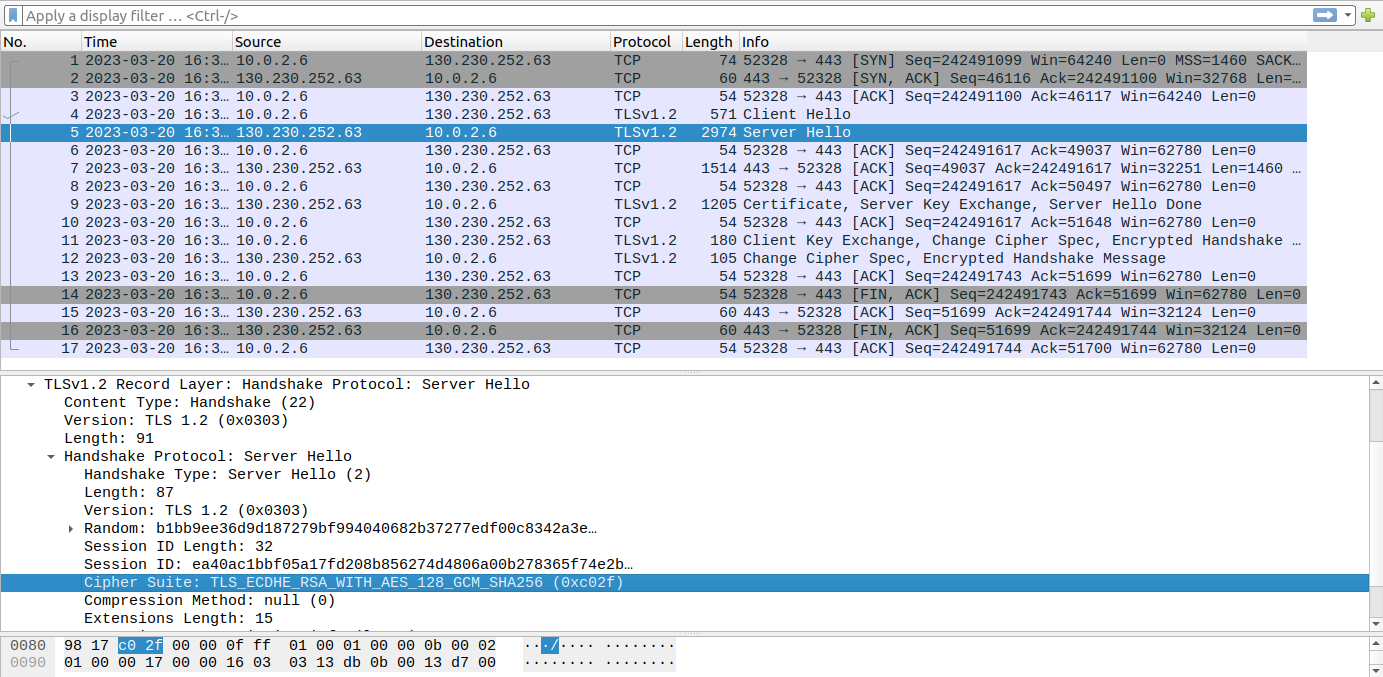
\includegraphics[height=\textheight,width=\textwidth,keepaspectratio]
    {figures/server_hello.png}
    \caption{`Server Hello' message of a TLS handshake.}
    \label{fig:server_hello_handshake}
\end{figure}

\begin{figure}
    \centering
    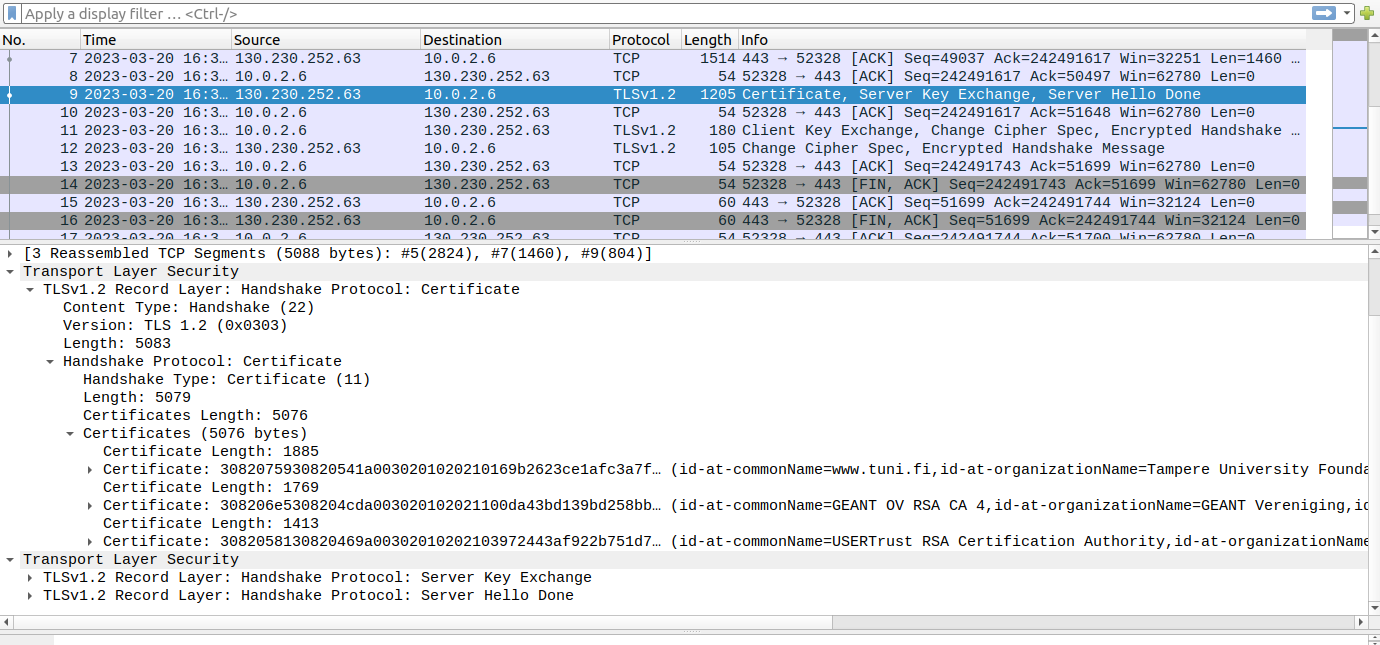
\includegraphics[height=\textheight,width=\textwidth,keepaspectratio]
    {figures/certificate_tls.png}
    \caption{`Certificate' segment of a TLS handshake.}
    \label{fig:cert_tls}
\end{figure}

Next, the TLS 1.2 handshake protocol started. Firstly, The client sent `Client Hello' message to
initiate the handshake. In this message, the client include its supported TLS version, supported
cipher suites (31 suites in this case), and a random number (see \autoref{fig:client_hello_handshake}). Next, the server
responded with a `Server Hello' message which contains the selected cipher suite and a
random number generated by the server (see \autoref{fig:server_hello_handshake}). Along with
that, the server also sent `Certificate', `Server Key Exchange', and `Server Hello Done'
messages. In the `Certificate' segment, information of SSL certifcates for verification were inlcuded
. As shown in \autoref{fig:cert_tls}, there are up to 3 certificates for verifying each other.
The reason is that a certificate of a web server is signed by an issuer A, and the certificate
of the issuer A is signed by a issuer B, and so forth until a certificate of the root CA is verified.
In each certificate, public-key elements (modulus, publicExponent, algorithm, etc.), subject, issuer,
etc. are included. In the `Server Key Exchange', parameters for Elliptic Curve Diffie-Hellman
Key Exchange (ECDKE) for exchanging the \emph{PreMasterSecret}, and the digital signature of
the message (see \autoref{fig:server_key_exchange_tls}).


\begin{figure}
    \centering
    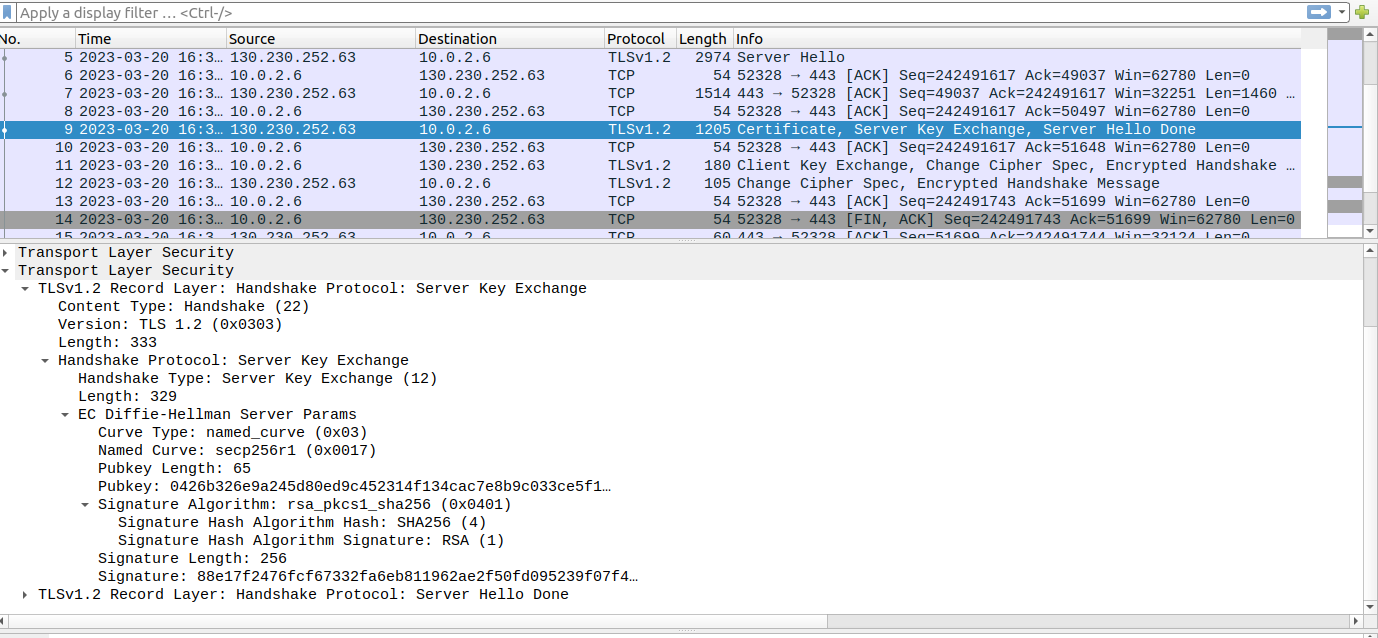
\includegraphics[height=\textheight,width=\textwidth,keepaspectratio]
    {figures/server_key_exchange.png}
    \caption{`Server Key Exchange' segment of a TLS handshake.}
    \label{fig:server_key_exchange_tls}
\end{figure}

\begin{figure}
    \centering
    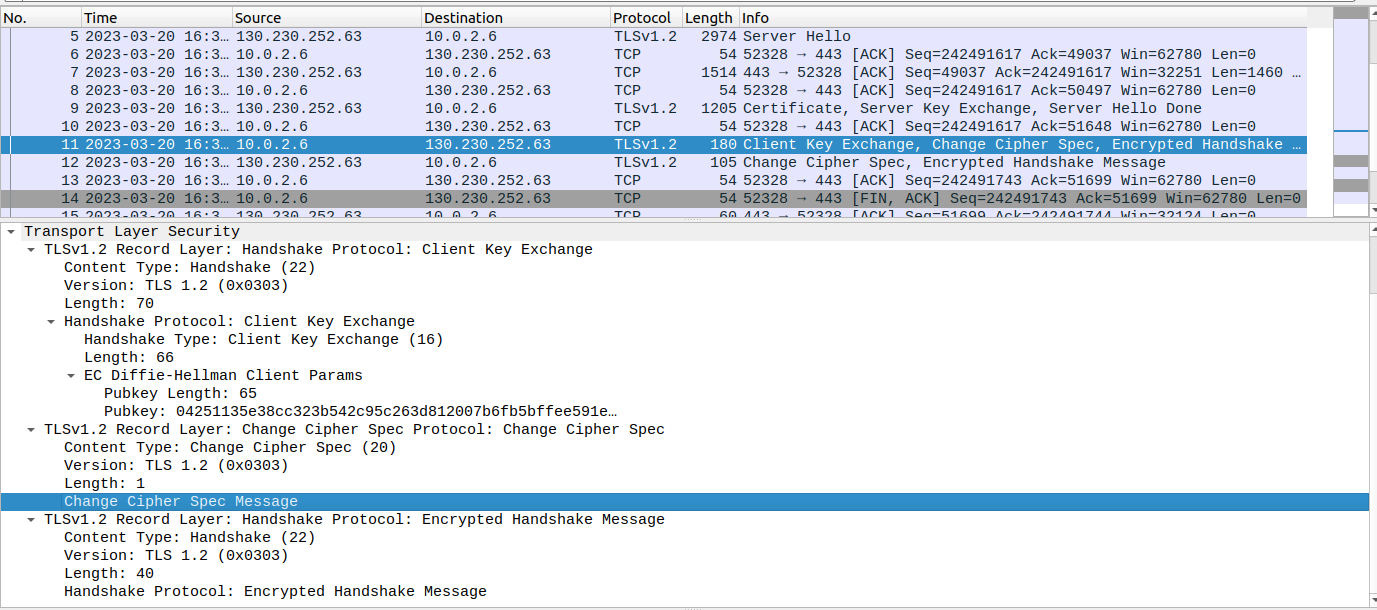
\includegraphics[height=\textheight,width=\textwidth,keepaspectratio]
    {figures/client_key_exchange.png}
    \caption{`Client Key Exchange', `Change Cipher Spec', and `Encrypted Handshake Message'
    segments of a TLS handshake from the client's side.}
    \label{fig:client_key_exchange_more_tls}
\end{figure}

\begin{figure}
    \centering
    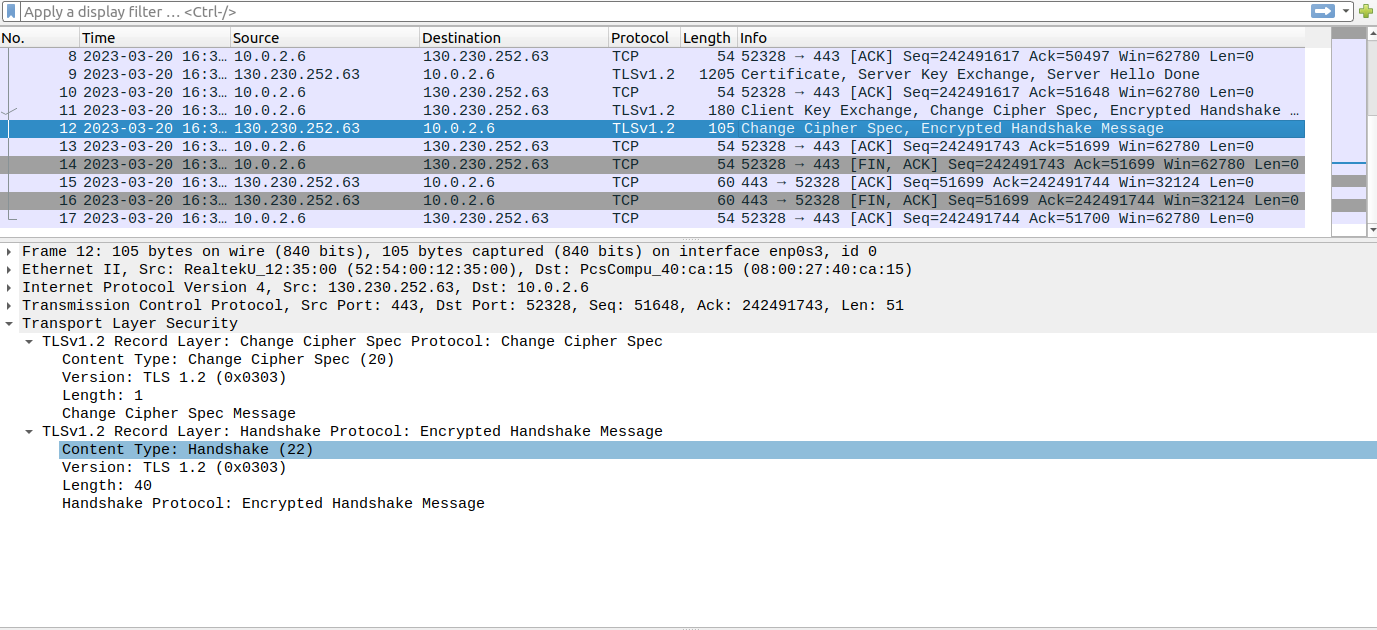
\includegraphics[height=\textheight,width=\textwidth,keepaspectratio]
    {figures/server_change_cipher_spec_more.png}
    \caption{`Change Cipher Spec' and `Encrypted Handshake Message' segments of a
    TLS handshake from the server's side.}
    \label{fig:server_change_cipher_spec_more_tls}
\end{figure}

Next, a `Server Hello Done' was sent to inform that the server had sent anything needed
for the next step. Then from the client's side, `Client Key Exchange', `Change Cipher Spec',
and `Encrypted Handshake Message' were replied (see \autoref{fig:client_key_exchange_more_tls}).
`Client Key Exchange' is replied, at this point,
the client and the server both have the same \emph{PreMasterSecret} which was combined with
random numbers generated in `Client Hello' and `Server Hello' to produce the \emph{MasterSecret},
a symmetric key used for later data encryption/decrytion. `Change Cipher Spec' from the client
informs that the client now had all information needed for starting encryption data. And
`Encrypted Handshake Message' is the encrypted message, with key is the \emph{MasterSecret},
that summerizes all of the messages in the handshake so far. Then, the server responded with
the same segments, `Change Cipher Spec' and `Encrypted Handshake Message'
(see \autoref{fig:server_change_cipher_spec_more_tls}). So at this point,
the TLS 1.2 handshake protocol was finished, data packets between the server and the client
later will be encrypted with the pre-agreed parameters and cryptographic algorithms.

%%%%%
\subsection{Task 1.b: CA's Certificate}
%%%%%

\begin{figure}[h!]
    \centering
    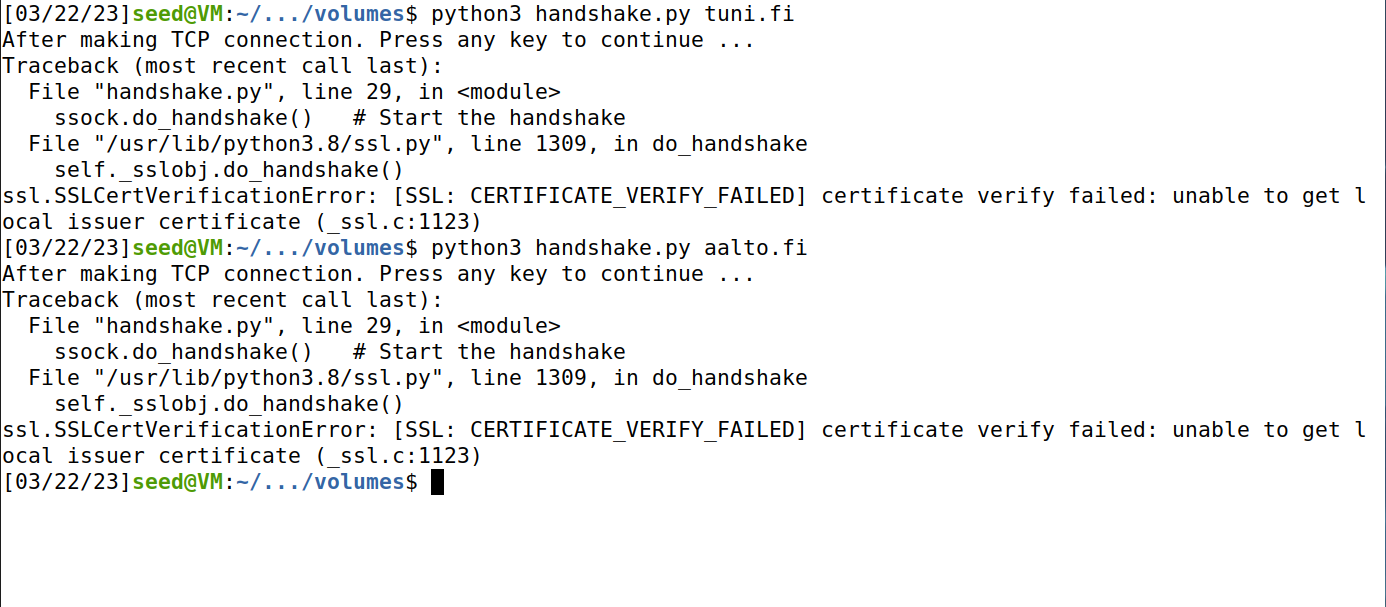
\includegraphics[height=\textheight,width=\textwidth,keepaspectratio]
    {figures/ssl_cert_verify_failed.png}
    \caption{SSl: Certificate verification falied.}
    \label{fig:cert_verify_failed}
\end{figure}

In this task, I did experiments with two websites: \url{www.tuni.fi} and \url{www.aalto.fi}.
These two web servers require different CA certificates. Without proper CA certificates
in the \url{./client-certs}, {\fontfamily{qcr}\selectfont handshake.py} raised an error
of ssl certificate verification (see \autoref{fig:cert_verify_failed}).

In the case of \url{www.tuni.fi}, at the first time I ran {\fontfamily{qcr}\selectfont
handshake.py} without changing the {\fontfamily{qcr}\selectfont cadir}, I noticed that
the issuer of its certificate is `USERTrust RSA Certification Authority'. So I went to
\url{/etc/ssl/certs} and found CA certificate named
\emph{USERTrust\_RSA\_Certification\_Authority.pem}. Then I copied this certificate to
\url{./client-certs}, and made a symbolic link to it, resulting a hash value
{\fontfamily{qcr}\selectfont fc5a8f99} (see \autoref{fig:ca_cert_client}). At this point,
a TLS handshake should be operated correctly as shown in \autoref{lst:handshake_log}.

On the other hand, in the case of \url{www.aalto.fi}, by the same way as above, I noticed
that the issuer of its certificate is `USERTrust ECC Certification Authority'. So I copied
\emph{USERTrust\_ECC\_Certification\_Authority.pem} from \url{/etc/ssl/certs} to
\url{./client-certs}, and made a symbolic link to it, resulting a hash value
{\fontfamily{qcr}\selectfont f30dd6ad} (see \autoref{lst:handshake_aalto})

\begin{figure}[h]
    \centering
    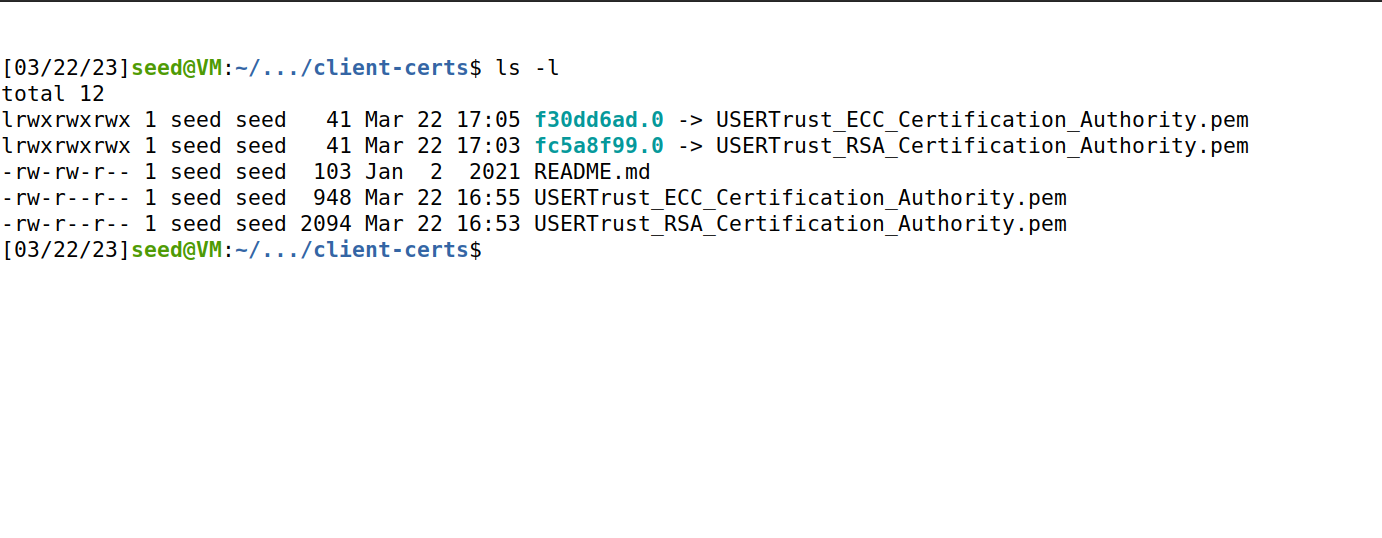
\includegraphics[width=\textwidth,height=\textheight,keepaspectratio]
    {figures/list_of_client_cert.png}
    \caption{List of CA certificates at the client side.}
    \label{fig:ca_cert_client}
\end{figure}

\begin{lstlisting}[language=bash, caption= A TLS handshake connecting to
    \url{www.aalto.fi}., label={lst:handshake_aalto}][h!]
$ python3 handshake.py aalto.fi
After making TCP connection. Press any key to continue ...
=== Cipher used: ('TLS_AES_256_GCM_SHA384', 'TLSv1.3', 256)
=== Server hostname: aalto.fi
=== Server certificate:
{'OCSP': ('http://GEANT.ocsp.sectigo.com',),
 'caIssuers': ('http://GEANT.crt.sectigo.com/GEANTOVECCCA4.crt',),
 'crlDistributionPoints': ('http://GEANT.crl.sectigo.com/GEANTOVECCCA4.crl',),
 'issuer': ((('countryName', 'NL'),),
            (('organizationName', 'GEANT Vereniging'),),
            (('commonName', 'GEANT OV ECC CA 4'),)),
 'notAfter': 'Oct 11 23:59:59 2023 GMT',
 'notBefore': 'Oct 11 00:00:00 2022 GMT',
 'serialNumber': 'B84AFD49576B21A3F25F63EBB683198C',
 'subject': ((('countryName', 'FI'),),
             (('stateOrProvinceName', 'Uusimaa'),),
             (('organizationName', 'Aalto University Foundation sr'),),
             (('commonName', 'aalto.fi'),)),
 'subjectAltName': (('DNS', 'aalto.fi'),
                    ('DNS', '5g-research.aalto.fi'),
                    ('DNS', 'abe.aalto.fi'),
                    ('DNS', 'accounting.aalto.fi'),
                    ('DNS', 'acre.aalto.fi'),
                    ('DNS', 'act.aalto.fi'),
                    ('DNS', 'aef.aalto.fi'),
                    ('DNS', 'aiic.aalto.fi'),
                    ('DNS', 'alumni.aalto.fi'),
                    ('DNS', 'ani.aalto.fi'),
                    ('DNS', 'architecture.aalto.fi'),
                    ('DNS', 'artcoordination.aalto.fi'),
                    ('DNS', 'arts.aalto.fi'),
                    ('DNS', 'asci.aalto.fi'),
                    ('DNS', 'avoin.aalto.fi'),
                    ('DNS', 'batcircle.aalto.fi'),
                    ('DNS', 'beta.aalto.fi'),
                    ('DNS', 'bimforlean.aalto.fi'),
                    ('DNS', 'bio2.aalto.fi'),
                    ('DNS', 'bioeconomy.aalto.fi'),
                    ('DNS', 'biofilia.aalto.fi'),
                    ('DNS', 'biz.aalto.fi'),
                    ('DNS', 'brainscience.aalto.fi'),
                    ('DNS', 'builtenv.aalto.fi'),
                    ('DNS', 'campusmember.aalto.fi'),
                    ('DNS', 'cearctic.aalto.fi'),
                    ('DNS', 'cemat.aalto.fi'),
                    ('DNS', 'chem.aalto.fi'),
                    ('DNS', 'choicetank.aalto.fi'),
                    ('DNS', 'civileng.aalto.fi'),
                    ('DNS', 'ckir.aalto.fi'),
                    ('DNS', 'cluster2017.aalto.fi'),
                    ('DNS', 'cmat.aalto.fi'),
                    ('DNS', 'cmet.aalto.fi'),
                    ('DNS', 'comnet.aalto.fi'),
                    ('DNS', 'comp.aalto.fi'),
                    ('DNS', 'copyright.aalto.fi'),
                    ('DNS', 'cqe.aalto.fi'),
                    ('DNS', 'cs.aalto.fi'),
                    ('DNS', 'datahub.aalto.fi'),
                    ('DNS', 'ddi.aalto.fi'),
                    ('DNS', 'design.aalto.fi'),
                    ('DNS', 'digi.aalto.fi'),
                    ('DNS', 'digital.aalto.fi'),
                    ('DNS', 'economics.aalto.fi'),
                    ('DNS', 'educase.aalto.fi'),
                    ('DNS', 'eea.aalto.fi'),
                    ('DNS', 'ele.aalto.fi'),
                    ('DNS', 'elec.aalto.fi'),
                    ('DNS', 'elo.aalto.fi'),
                    ('DNS', 'energy.aalto.fi'),
                    ('DNS', 'energyscience.aalto.fi'),
                    ('DNS', 'eng.aalto.fi'),
                    ('DNS', 'facilityrental.aalto.fi'),
                    ('DNS', 'ficore.aalto.fi'),
                    ('DNS', 'fif.aalto.fi'),
                    ('DNS', 'finance.aalto.fi'),
                    ('DNS', 'globalimpact.aalto.fi'),
                    ('DNS', 'health.aalto.fi'),
                    ('DNS', 'hema.aalto.fi'),
                    ('DNS', 'hyber.aalto.fi'),
                    ('DNS', 'icetank.aalto.fi'),
                    ('DNS', 'information.aalto.fi'),
                    ('DNS', 'innovation.aalto.fi'),
                    ('DNS', 'inside.aalto.fi'),
                    ('DNS', 'it.aalto.fi'),
                    ('DNS', 'lifewidelearning.aalto.fi'),
                    ('DNS', 'living.aalto.fi'),
                    ('DNS', 'lounasmaalab.aalto.fi'),
                    ('DNS', 'ltl.aalto.fi'),
                    ('DNS', 'ltq.aalto.fi'),
                    ('DNS', 'luma.aalto.fi'),
                    ('DNS', 'lwl.aalto.fi'),
                    ('DNS', 'management.aalto.fi'),
                    ('DNS', 'marketing.aalto.fi'),
                    ('DNS', 'materials.aalto.fi'),
                    ('DNS', 'mechatronics.aalto.fi'),
                    ('DNS', 'mecheng.aalto.fi'),
                    ('DNS', 'media.aalto.fi'),
                    ('DNS', 'medialab.aalto.fi'),
                    ('DNS', 'metsahovi.aalto.fi'),
                    ('DNS', 'nbe.aalto.fi'),
                    ('DNS', 'nmc.aalto.fi'),
                    ('DNS', 'npharvest.aalto.fi'),
                    ('DNS', 'openaccess.aalto.fi'),
                    ('DNS', 'otanano.aalto.fi'),
                    ('DNS', 'ourblogs.aalto.fi'),
                    ('DNS', 'pati.aalto.fi'),
                    ('DNS', 'physics.aalto.fi'),
                    ('DNS', 'promootio.aalto.fi'),
                    ('DNS', 'rawmaterials.aalto.fi'),
                    ('DNS', 'sci.aalto.fi'),
                    ('DNS', 'sem.aalto.fi'),
                    ('DNS', 'shakinguptech.aalto.fi'),
                    ('DNS', 'spa.aalto.fi'),
                    ('DNS', 'spacecraft.aalto.fi'),
                    ('DNS', 'startupcenter.aalto.fi'),
                    ('DNS', 'taide.aalto.fi'),
                    ('DNS', 'test.content.aalto.fi'),
                    ('DNS', 'test.datahub.aalto.fi'),
                    ('DNS', 'test.lifewidelearning.aalto.fi'),
                    ('DNS', 'test.ourblogs.aalto.fi'),
                    ('DNS', 'tuta.aalto.fi'),
                    ('DNS', 'uwas.aalto.fi'),
                    ('DNS', 'virtualexhibitions.aalto.fi'),
                    ('DNS', 'www.aalto.fi')),
 'version': 3}
[{'issuer': ((('countryName', 'US'),),
             (('stateOrProvinceName', 'New Jersey'),),
             (('localityName', 'Jersey City'),),
             (('organizationName', 'The USERTRUST Network'),),
             (('commonName', 'USERTrust ECC Certification Authority'),)),
  'notAfter': 'Jan 18 23:59:59 2038 GMT',
  'notBefore': 'Feb  1 00:00:00 2010 GMT',
  'serialNumber': '5C8B99C55A94C5D27156DECD8980CC26',
  'subject': ((('countryName', 'US'),),
              (('stateOrProvinceName', 'New Jersey'),),
              (('localityName', 'Jersey City'),),
              (('organizationName', 'The USERTRUST Network'),),
              (('commonName', 'USERTrust ECC Certification Authority'),)),
  'version': 3}]

\end{lstlisting}